\section{Heap Allocation}

In this section we consider a small experiment to investigate possible differences in heap fragmentation caused by dynamic allocation in {\C} and {\rust}.
The conducted experiment is a simple program which allocates 128 objects on the heap.
Then in a loop with 1024 iterations, one object is chosen each iteration and replaced with a new object.
The objects are of the three sizes given in \autoref{tab:heap:objects}.

\begin{table}[H]
  \centering
  \begin{tabular}{l|l|l}
    \textbf{Name} & \textbf{Size (32-bit words)} & \textbf{Color} \\
    \hline
    A & 2 & Green \\
    B & 3 & Red \\
    C & 6 & Blue \\
    \hline
  \end{tabular}
  \caption{}
  \label{tab:heap:objects}
\end{table}

The heap allocation pattern was recorded after the initial 128 objects were allocated and are given in \autoref{fig:heap:init}.
We see that the initial allocation pattern is alternating between these three object sizes, and the white space between is padding due to alignment rules of the allocator.
The objects are created in the same order in both {\C} and {\rust} and we see that the allocation patterns are identical, as expected.

\begin{figure}[H]

  \centering
  \begin{subfigure}{0.47\textwidth}
    \centering
    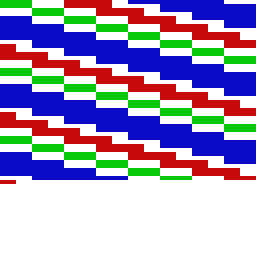
\includegraphics[scale=0.25]{results/plots/heap/cinit}
    \caption{C}
    \label{fig:heap:init:c}
  \end{subfigure}
  \hfill
  \begin{subfigure}{0.47\textwidth}
      \centering
    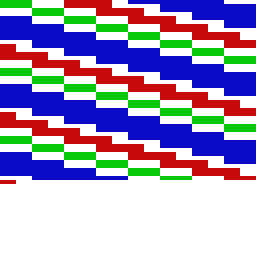
\includegraphics[scale=0.25]{results/plots/heap/rinit}
    \caption{Rust}
    \label{fig:heap:init:r}
  \end{subfigure}
  \caption{Initial heap allocation of 128 objects in {\rust} and {\C}}
  \label{fig:heap:init}

\end{figure}

During the 1024 iterations, the objects are replaced in a psudo random manner.
To get comparable results for both {\C} and {\rust} the random number generator used, is the same for both languages (this is the same \gls{rng} as discussed in \autoref{sec:res:perf}).
\autoref{fig:heap:frag} presents the heap allocation pattern after the loop has been executed.
From this figure, we see that the allocation patterns in {\rust} and {\C} are identical.

\begin{figure}[H]

  \centering
  \begin{subfigure}{0.47\textwidth}
    \centering
    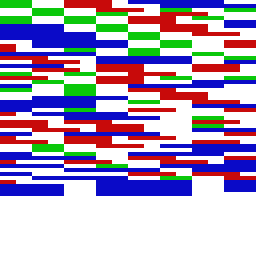
\includegraphics[scale=0.25]{results/plots/heap/cfrag}
    \caption{C}
    \label{fig:heap:frag:c}
  \end{subfigure}
  \hfill
  \begin{subfigure}{0.47\textwidth}
      \centering
    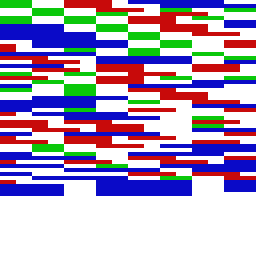
\includegraphics[scale=0.25]{results/plots/heap/rfrag}
    \caption{Rust}
    \label{fig:heap:frag:r}
  \end{subfigure}
  \caption{Heap allocation after processing in {\rust} and {\C}}
  \label{fig:heap:frag}

\end{figure}
